\documentclass{article}
\usepackage[utf8]{inputenc}
\usepackage{geometry}
\usepackage{csquotes}
\usepackage[portuguese]{babel}
\usepackage[pdftex]{hyperref}
\usepackage{indentfirst}
\usepackage{tcolorbox}
\usepackage{amsmath}
\usepackage{tikz}
\usepackage{float}
\usepackage{amsfonts}
\usepackage{listings}
\usepackage{xcolor}

\definecolor{codegreen}{rgb}{0,0.6,0}
\definecolor{codegray}{rgb}{0.5,0.5,0.5}
\definecolor{codepurple}{rgb}{0.58,0,0.82}
\definecolor{backcolour}{rgb}{0.95,0.95,0.92}

\lstdefinestyle{mystyle}{
    backgroundcolor=\color{backcolour},   
    commentstyle=\color{codegreen},
    keywordstyle=\color{magenta},
    numberstyle=\tiny\color{codegray},
    stringstyle=\color{codepurple},
    basicstyle=\ttfamily\footnotesize,
    breakatwhitespace=false,         
    breaklines=true,                 
    captionpos=b,                    
    keepspaces=true,                 
    numbers=left,                    
    numbersep=5pt,                  
    showspaces=false,                
    showstringspaces=false,
    showtabs=false,                  
    tabsize=2
}

\lstset{style=mystyle}

\tikzstyle{node} = [circle, draw = blue!50, fill = blue!20, thick, inner sep = 0pt, minimum size = 6mm]

\newtcolorbox{mybox}[3][]
{
  colframe = #2!25,
  colback  = #2!10,
  coltitle = #2!20!black,  
  title    = {#3},
  #1,
}

\geometry{top = 3cm, bottom = 2cm, right = 2cm, left = 3cm}

\title{PageRank e Cadeias de Markov}
\author{Cristhian Grundmann \\
Hanna Rodrigues Ferreira \\
Igor Cortes Junqueira \\
Igor Patrício Michels}

\date{Dezembro de 2021}

\begin{document}

\maketitle

\section*{Introdução}

Imagine que você esteja curioso acerca de um determinado tema, o que você faz? Se a resposta é ``dou um Google'', parabéns, você acaba de utilizar o algoritmo PageRank! Criado oficialmente em agosto de 1998, a Google surgiu com uma ideia de Larry Page e Sergey Brin. A história se inicia em 1995, quando Page foi conhecer a universidade de Stanford e Brin recebeu a tarefa de mostrar a universidade para ele. No início os dois discordavam sobre muita coisa mas, no ano seguinte, fecharam uma parceria visando criar um mecanismo de busca que pudesse ``organizar as informações do mundo e torná-las universalmente acessíveis e úteis''. Para isso, desenvolveram um algoritmo que usava os links para determinar a importância de cada página da internet \cite{google}.

Rapidamente o mecanismo ganhou força, virando o principal mecanismo de buscas. Esse fato se dá por que as estratégias de calcular a relevância, até o momento, eram calculadas usando apenas os dados da própria página, algo que poderia ser facilmente burlado e, com isso, poderia deixar resultados pouco relevantes nas primeiras posições, principalmente com o grande crescimento da internet na época.

\section*{Cadeias de Markov}

Cadeias de Markov são um modelo estocástico que descreve uma sequência de eventos onde a probabilidade dos mesmos só depende do estado anterior. Esses modelos podem ser aplicados em tempo discreto ou continuo, e são usados para diversos processos como filas ou dinâmica populacional animal. Processos de Markov são a base para simulações do tipo 'Monte Carlo Markov Chain', que podem ser usados para amostrar de distribuições de probabilidade complexas, com aplicações em diversas áreas.

Cadeias de Markov podem ser representadas de forma simples por uma 'matriz de transição', que descreve as probabilidades de transição de cada estado em particular para os demais possíveis estados. Com essa modelagem, torna-se fácil manipular computacionalmente o processo. Também é possível obter resultados como a chamada 'distribuição estacionária', que representa uma especie de 'equilíbrio' no processo a longo prazo, onde é conhecida a representatividade de cada estado no todo. Se a Cadeia de Markov em questão é 'não periódica', o que pode ser entendido como não haver ciclos de forma a limitar as transições a múltiplos fixos de passos para cada estado, podemos garantir existência e unicidade da distribuição estacionária.

\subsubsection*{O teorema de Perron-Frobenius}

O Teorema de Perron-Frobenius afirma, resumidamente, que uma matriz $d \times d$ de elementos positivos possui um autovalor positivo com multiplicidade algébrica um e é o maior autovalor em módulo. No nosso caso, isso é particularmente útil por garantir que uma matriz de transição de estados possua um autovetor correspondente ao autovalor $1$, sendo justamente o estado estacionário do processo modelado, além de garantir a unicidade do mesmo.

\noindent
\textbf{Teorema de Perron-Frobenius}: Seja $A$ uma matriz $d \times d$ de entradas positivas, isto é $A_{ij}>0$ $\forall i, j = 1, \dots, d$. Então:

\begin{enumerate}
    \item $A$ possui um único autovetor $x$ de norma $1$, cujas componentes são, todas elas, positivas;
    \item o autovalor $\lambda_+$ associado ao autovetor $x$ é positivo e, para qualquer outro autovalor $\lambda \in \mathbb{C}$, temos que $|\lambda| < \lambda_+$;
    \item o autovalor $\lambda_+$ é simples;
\end{enumerate}

A prova dos itens desse teorema se dão, dentre outras abordagens, por álgebra linear. Detalhes dessa demostração não serão abordadas nesse texto por conveniência, já que se estende ao escopo do trabalho. A comprovação completa pode ser encontrada detalhadamente na seção 2 de \cite{perron-frobenius}.

\section*{PageRank}

Indo um pouco na contramão de algumas outras estratégias, o PageRank visa calcular a relevância de uma página por meio de fatores externos. De maneira simples, podemos usar um grafo para ilustrar uma pequena rede, onde os nós são os sites e as arestas, direcionadas, representam que o site de origem tem um link para o site de destino. É esperado que o site que receba a maior quantidade de links (maior grau de entrada) deve ser o mais relevante, mas e em caso de empate? A ideia de Page e Brin foi ponderar os votos de acordo com a relevância, isso é, se um site tem uma alta relevância, seu voto deve ter um peso maior que o voto de um site que não recebe link algum.
\begin{mybox}{green}{Exemplo}
    Um site que recebe apenas um link, mas do G1, deve ser mais relevante que um site que recebe apenas um link de um site pessoal.
\end{mybox}

\subsection*{Conexão com as Cadeias de Markov}

Intuitivamente, podemos pensar no processo de um internauta ficar navegando na internet e trocar de sites por meio de links presentes no próprio site, com mesma probabilidade para cada link. Dessa forma, se um site $S$ tem link para $n$ diferentes sites ($T_1$, $T_2$, $\dots$ e $T_n$), a probabilidade do internauta sair do site $S$ para os sites $T_i, i \in \{1, 2, \dots, n\}$ é igual a $\frac{1}{n}$ e é nula para qualquer outro site. Note que temos uma modelagem concisa que representa a rede de modo simples resta, então, definir uma métrica para representar a relevância de um site.

Pensando em Cadeias de Markov, e em sua evolução temporal, podemos pensar que uma boa métrica seja dada pela proporção do tempo que o internauta aleatório passa em cada site ao realizar um passeio aleatório pelos mesmos. Ou seja, vamos dizer que a relevância é maior para sites mais recorrentes e menor para os menos visitados. Dessa forma, podemos ver que sites que são muito linkados tendem a aparecer mais vezes no passeio. Consequentemente, os que são linkados pelos mais recorrentes também tendem a aparecer mais vezes. Já os sites pouco linkados e com links de sites menos recorrentes tendem a aparecer por menos tempo no passeio.

Note que essas propriedades são justamente as desejáveis para nosso ranking, ou seja, estamos com uma métrica em que os sites mais bem colocados tenham votos com peso maior que os piores colocados. Por fim, temos que a relevância pode ser calculada por meio do vetor estacionário da Cadeia de Markov definida pela rede.

\subsection*{Alguns problemas da modelagem}

Vamos supor que uma sub-rede da nossa rede seja cíclica, como na Figura \ref{graph1}. Se executarmos o passeio aleatório definido anteriormente temos que, se um internauta cair dentro desse ciclo, em $A$, por exemplo, ele ficará seguindo o caminho $A\to B\to C\to A$ infinitamente. Dessa forma, podemos ver que, ao entrar no ciclo, o tempo que o internauta permanece em cada site desse ciclo é $\frac{1}{3}$, o que nos daria igual relevância a cada um dos três sites do ciclo e relevância zero para os demais sites da rede, o que seria problemático.

Outro exemplo pode ser visto na Figura \ref{graph2}, onde temos a aparição de um nó terminal. Note que, num passeio aleatório, se um internauta acessa o site $G$, ele permanece nele infinitamente, o seja, teremos relevância $1$ para o site $G$ e zero para os demais, o que também seria um problema.
\begin{figure}[H]
    \centering
    \begin{minipage}{.5\textwidth}
        \centering
        \begin{tikzpicture}
            \node (A) at (0, 1.7) [node] {A};
            \node (B) at (-1, 0) [node] {B};
            \node (C) at (1, 0) [node] {C};
            \draw [->, line width = 0.25mm] (A) -- (B);
            \draw [->, line width = 0.25mm] (B) -- (C);
            \draw [->, line width = 0.25mm] (C) -- (A);
        \end{tikzpicture}
        \caption{Exemplo de rede cíclica.}
        \label{graph1}
    \end{minipage}%
    \begin{minipage}{.5\textwidth}
        \centering
        \begin{tikzpicture}
            \node (D) at (5, 2.55) [node] {D};
            \node (E) at (5, 0.85) [node] {E};
            \node (F) at (5, -0.85) [node] {F};
            \node (G) at (7, 0.85) [node] {G};
            \draw [->, line width = 0.25mm] (D) -- (G);
            \draw [->, line width = 0.25mm] (E) -- (G);
            \draw [->, line width = 0.25mm] (F) -- (G);
        \end{tikzpicture}
        \caption{O nó G é um nó terminal.}
        \label{graph2}
    \end{minipage}
\end{figure}

\subsection*{Solucionando os problemas}

Para driblar esses problemas podemos fazer algumas adaptações nas redes, alterando um pouco a estrutura e as probabilidades, mas visando uma maior coerência e correção desses problemas. A alteração estrutural se dará pela inserção de arestas de modo que o grafo fique completo, com todos os nós apontando para todos os outros nós. Quanto as probabilidades, fixaremos um valor $p\in (0, 1)$ e a matriz de transição dessa nova Cadeia será dada por
\[\tilde{M} = (1 - p)\cdot M + p\cdot \dfrac{I}{n},\]

\noindent onde temos
\begin{itemize}
    \item
        $\tilde{M}$: a matriz de transição da nova cadeia;
        
    \item
        $M$: a matriz de transição da cadeia original;
        
    \item
        $I$: a matriz de uns de tamanho $n\times n$ e;
        
    \item
        $n$: o número de nós da rede.
\end{itemize}

Visualmente, podemos ilustrar os grafos anteriores após as alterações como na Figura \ref{graph12}. Na rede da esquerda, as arestas azuis representam as próprias arestas, enquanto as vermelhas representam grupos de arestas que se conectam a cada uma das arestas da outra parte do grafo, representada no Grafo.
\begin{figure}[H]
    \centering
    \begin{tikzpicture}
        \node (A) at (0, 1.7) [node] {A};
        \node (B) at (-1, 0) [node] {B};
        \node (C) at (1, 0) [node] {C};
        \node (Graph) at (0, 3) [node] {Grafo};
        \draw [->, line width = 0.25mm] (A) -- (B);
        \draw [<-, dashed, blue] (A) to[out = 180, in = 180] (B);
        \draw [->, line width = 0.25mm] (B) -- (C);
        \draw [<-, dashed, blue] (B) to[out = -90, in = -90] (C);
        \draw [->, line width = 0.25mm] (C) -- (A);
        \draw [<-, dashed, blue] (C) to[out = 0, in = 0] (A);
        \draw [->, line width = 0.25mm] (Graph) -- (A);
        \draw [<->, dashed, red] (C) to[out = 45, in = 45] (Graph);
        \draw [<->, dashed, red] (B) to[out = 135, in = 180] (Graph);
        \draw [<->, dashed, red] (A) to[out = 45, in = 0] (Graph);
    
        \node (D) at (5, 2.55) [node] {D};
        \node (E) at (5, 0.85) [node] {E};
        \node (F) at (5, -0.85) [node] {F};
        \node (G) at (7, 0.85) [node] {G};
        \draw [->, line width = 0.25mm] (D) -- (G);
        \draw [->, line width = 0.25mm] (E) -- (G);
        \draw [->, line width = 0.25mm] (F) -- (G);
        
        \draw [<->, dashed, blue] (D) -- (E);
        \draw [<->, dashed, blue] (E) -- (F);
        \draw [<->, dashed, blue] (D) to[out = 180, in = 180] (F);
        \draw [->, dashed, blue] (G) to[out = 90, in = 0] (D);
        \draw [->, dashed, blue] (G) to[out = 157.5, in = 22.5] (E);
        \draw [->, dashed, blue] (G) to[out = -90, in = 00] (F);
    \end{tikzpicture}
    \caption{Grafos anteriores após alteração descrita.}
    \label{graph12}
\end{figure}

Uma interpretação dessa alteração é a de que o processo ocorre com o internauta, antes de sair do site, jogando uma moeda de probabilidade $p$ para sair cara. Saindo cara, o internauta vai na barra de endereços e digita o endereço de qualquer site (podendo inclusive digitar o endereço do site atual) com mesma probabilidade, acessando o site que foi digitado na barra de endereços. Já se a moeda der coroa, então o internauta entra em um dos links da página, novamente com a mesma probabilidade entre os links existentes.

Podemos perceber que, com essas alterações, os problemas de ficarmos presos num ciclo ou num nó terminal acabam, pois temos uma probabilidade positiva de ir a outro nó da rede. Por fim, note também que essa alteração fez a matriz $\tilde{M}$ ser positiva o que, pelo Teorema de Perron-Frobenius, diz que essa matriz possui um estado estacionário $\pi$.

\section*{Implementações Computacionais}

Nessa seção iremos comentar acerca da parte computacional do tema, isso é, sobre a implementação do PageRank em Python e uma simulação em C.

\subsection*{Cálculo do PageRank}

\subsubsection*{Solução via Sistema Linear}

Lembrando que, como comentado anteriormente, o PageRank pode ser visto como o autovetor correspondente ao autovalor $1$ da matriz $\tilde{M}$, como definida anteriormente. Dessa forma, podemos calcular o PageRank por meio da resolução de um sistema linear do tipo $I - (1 - p)\cdot A^\top = b$, onde $A$ é a matriz de adjacências do grafo correspondente, já normalizada por linha e $b$ é um vetor de coluna com $n$ linhas e todas as entradas sendo iguais a $\frac{p}{n}$. Uma implementação para isso pode ser vista na Listing \ref{sistema}, onde a entrada é a matriz de adjacências de um grafo e o valor $p$ correspondente a probabilidade de um salto aleatório.

\begin{lstlisting}[language = Python, caption = Algoritmos para calcular a integral dada de modo aproximado., label = sistema]
import numpy as np
from numpy.linalg import solve

def PageRank(A, p):
    A = np.array(A, dtype = np.float64)
    for i in range(A.shape[0]):
        soma = sum(A[i, :])
        for j in range(A.shape[1]):
            A[i, j] = A[i, j]/soma
    
    A = A.T
    n = A.shape[1]
    A = np.eye(n, n) - (1 - p) * A
    b = p * (np.ones(n, dtype = np.float64) / n)
    
    return solve(A, b)
\end{lstlisting}

\subsubsection*{Solução via Método da Potência}

Uma outra forma de encontrar o PageRank é usar sua interpretação de vetor estacionário, ou seja, um vetor $\pi$ tal que $M\pi = \pi$. Dessa forma, podemos pensar em encontrar o PageRank de uma rede por meio de um processo iterativo onde aplicamos a matriz $\tilde{M}$ várias vezes a um vetor inicial, até que ocorra a convergência. Essa ideia pode ser vista na Listing \ref{potencia}, onde a função recebe a matriz $A$, matriz de adjacências do grafo correspondente, $p$, a probabilidade de salto aleatório, e $tol$, uma tolerância para a convergência. Na função calculamos a matriz $\tilde{M}$ e aplicamos ela no vetor $e_1$ até que ocorra a convergência.

\begin{lstlisting}[language = Python, caption = Algoritmos para calcular a integral dada de modo aproximado., label = potencia]
import numpy as np
from numpy.linalg import norm

def PageRank(A, p, tol = 1e-10):
    A = np.array(A, dtype = np.float64)
    for i in range(A.shape[0]):
        soma = sum(A[i, :])
        for j in range(A.shape[1]):
            A[i, j] = A[i, j]/soma
            
    n = A.shape[0]
    A = (1 - p) * A + p * np.ones((n, n)) / n
    
    v0 = np.zeros(n, dtype = np.float64)
    v0[0] = 1
    v1 = v0 @ A
    while norm(v1 - v0) > tol:
        v0 = v1
        v1 = v0 @ A
        
    return v1
\end{lstlisting}

\subsubsection*{Exemplo}

Os códigos acima foram testados na rede da Figura \ref{exemplo}, com $p = 0.15$. Note que a matriz de adjacências correspondente é dada por
\[A = \begin{bmatrix}0 & 1 & 1 & 1 & 1 \\ 1 & 0 & 1 & 1 & 1 \\ 1 & 1 & 0 & 1 & 1 \\ 1 & 1 & 1 & 0 & 1 \\ 0 & 0 & 0 & 0 & 1\end{bmatrix},\]

\noindent nos dando as matrizes
\[A = \begin{bmatrix}1 & -0.2125 & -0.2125 & -0.2125 & 0 \\ -0.2125 & 1 & -0.2125 & -0.2125 & 0 \\ -0.2125 & -0.2125 & 1 & -0.2125 & 0 \\ -0.2125 & -0.2125 & -0.2125 & 1 & 0 \\ -0.2125 & -0.2125 & -0.2125 & -0.2125 & 0.15\end{bmatrix}\text{ e }\tilde{M} = \begin{bmatrix}0.03 & 0.2425 & 0.2425 & 0.2425 & 0.2425 \\ 0.2425 & 0.03 & 0.2425 & 0.2425 & 0.2425 \\ 0.2425 & 0.2425 & 0.03 & 0.2425 & 0.2425 \\ 0.2425 & 0.2425 & 0.2425 & 0.03 & 0.2425 \\ 0.03 & 0.03 & 0.03 & 0.03 & 0.88\end{bmatrix},\]

\noindent correspondentes a resolução pelo sistema linear e pelo método da potência, respectivamente. Como resultado, temos que o PageRank dessa rede é $\begin{bmatrix}0.0827586 & 0.0827586 & 0.0827586 & 0.0827586 & 0.668966\end{bmatrix}$.

\begin{figure}[H]
    \centering
    \begin{tikzpicture}
        \node (0) at (3, 0) [node] {0};
        \node (1) at (0.9271, 2.8532) [node] {1};
        \node (2) at (-2.4271, 1.7634) [node] {2};
        \node (3) at (-2.4271, -1.7634) [node] {3};
        \node (4) at (0.9271, -2.8532) [node] {4};
        \draw [<->] (0) -- (1);
        \draw [<->] (0) -- (2);
        \draw [<->] (0) -- (3);
        \draw [->] (0) -- (4);
        \draw [<->] (1) -- (2);
        \draw [<->] (1) -- (3);
        \draw [->] (1) -- (4);
        \draw [<->] (2) -- (3);
        \draw [->] (2) -- (4);
        \draw [->] (3) -- (4);
    \end{tikzpicture}
    \caption{Exemplo de rede.}
    \label{exemplo}
\end{figure}

\subsection*{Simulação}

A simulação do PageRank funciona em uma rede de sites, que podem ter links para outros sites, exceto a si mesmos. Um site pode não ter links.

Cada site possui, inicialmente, uma certa quantidade de visitantes, possivelmente aleatória. A simulação consiste em iterações sobre o número de visitantes em cada site, onde o comportamento assintótico é o objeto de estudo. Para computar uma iteração, é tratado um site por vez. A ordem de tratamento não afeta o resultado final. Cada visitante faz um passo da cadeia de Markov associada ao PageRank, que funciona da seguinte forma:
\begin{itemize}
    \item com probabilidade p, o internauta escolhe um site aleatório entre todos os sites (salto), ignorando os links, com distribuição uniforme;
    \item caso contrário, escolhe um link do seu site atual aleatoriamente, novamente com distribuição uniforme. No caso do site não ter nenhum link, o visitante permanece no mesmo site.
\end{itemize}

Note que o visitante pode se manter no site no caso de um salto ou quando não há links para seguir a partir do site atual.

A implementação não é tão trivial, pois a quantidade de visitantes de um site não pode sofrer interferência de um site tratado anteriormente. Por exemplo, os visitantes do primeiro site podem ir para outros sites, mas quando estes forem tratados, os visitantes novos não podem ser contados, somente os antigos.

Para resolver isso, cada site possui, na verdade, duas variáveis para lembrar a quantidade de visitantes. Uma é primária e outra secundária. Quando um site é tratado, os visitantes atuais estão na variável primária e vão para a variável secundária nos seus destinos. No final do tratamento, a variável primária do site deve ser $0$, pois todos os visitantes do site foram tratados. Aqueles que continuam no mesmo site estão na variável secundária.

Após tratar todos os sites, os papéis das duas variáveis são trocados. Note que antes da iteração, todas as variáveis secundárias sempre são $0$, e é importante que haja uma inicialização adequada antes da primeira iteração.

O programa que implementa a simulação foi escrito em C, e usa a biblioteca GTK+3. A compilação foi testada apenas em sistemas Linux, e depende do pacote \texttt{libgtk-3-dev}, além do compilador C e do comando \texttt{make} provavelmente já instalado por padrão. A compilação pode ser feita usando o arquivo Makefile, rodando o comando \texttt{make}. O programa tem uma interface gráfica, como pode ser vista na Figura \ref{simulacao}. Nessa interface há uma região mostrando a rede, e uma região com 3 controles, o valor de $p$, o tempo das iterações, e o raio/escala dos elementos da rede. Há uma região que exibe um texto descrevendo os comandos para manipular a rede, bastando passar o mouse por cima.

\begin{figure}[H]
    \centering
    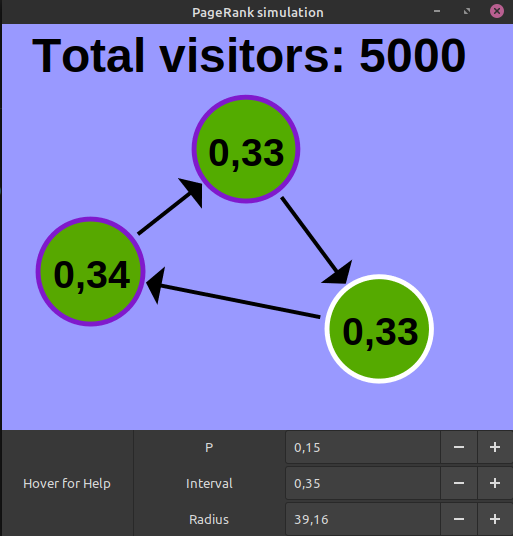
\includegraphics[scale = 0.35]{pagerank_demo.png}
    \caption{Interface gráfica do programa criado para ilustrar o PageRank.}
    \label{simulacao}
\end{figure}

\newpage
\begin{thebibliography}{9}

\bibitem{google} Como nós começamos e onde estamos hoje. \textit{Google}. \url{https://about.google/our-story/}.

\bibitem{usp} O algoritmo PageRank do Google. \textit{Miguel Frasson - ICMC/USP}. \url{https://edisciplinas.usp.br/pluginfile.php/5790758/mod_resource/content/1/pagerank-estat.pdf}.

\bibitem{wiki} ``PageRank''. \textit{Wikipedia}. \url{https://en.wikipedia.org/wiki/PageRank}.

\bibitem{perron-frobenius} O Teorema de Perron-Frobenius e a Ausência de Transição de Fase em Modelos Unidimensionais da Mecânica Estatíıstica. \textit{Marcelo Richard Hilário - UFMG. Gastão Braga - UFMG}. \url{https://www.ime.usp.br/~map2121/2014/map2121/programas/perron-frobenius.pdf}.

\end{thebibliography}

\end{document}

